\documentclass{book}

% Preamble - all your packages and settings
\usepackage{graphicx}
\usepackage{lipsum} % for placeholder text, remove in real project
\usepackage{authblk} % For better author formatting
\usepackage{array} % For better table formatting
\usepackage{booktabs} % For professional-looking tables
\usepackage{url} % For proper URL formatting
\usepackage{hyperref}
\usepackage{listings}
\usepackage{xcolor}
\usepackage{hyperref}
\usepackage{float} 
\usepackage{graphicx}
\graphicspath{{chapters/}}
\usepackage{float}
\usepackage{amssymb} 
\usepackage{ulem}
\usepackage{graphicx} 

% Configure lstlisting
\lstset{
  basicstyle=\ttfamily\footnotesize,
  breaklines=true,
  numbers=left,
  numberstyle=\tiny\color{gray},
  keywordstyle=\color{blue},
  commentstyle=\color{green!50!black},
  stringstyle=\color{orange},
  showstringspaces=false,
  frame=single,
  escapeinside={(*@}{@*)}
}
\usepackage{listings}
\usepackage{xcolor}

% Define colors for code
\definecolor{codegray}{rgb}{0.5,0.5,0.5}
\definecolor{codepurple}{rgb}{0.58,0,0.82}
\definecolor{backcolour}{rgb}{0.95,0.95,0.92}

% General code style
\lstdefinestyle{mystyle}{
    backgroundcolor=\color{backcolour},
    commentstyle=\color{codegray},
    keywordstyle=\color{blue},
    numberstyle=\tiny\color{codegray},
    stringstyle=\color{codepurple},
    basicstyle=\ttfamily\footnotesize,
    breaklines=true,
    captionpos=b,
    keepspaces=true,
    numbers=left,
    numbersep=5pt,
    showspaces=false,
    showstringspaces=false,
    showtabs=false,
    tabsize=2
}
\lstset{style=mystyle}

% Enable JavaScript
\lstdefinelanguage{JavaScript}{
  keywords={typeof, new, true, false, catch, function, return, null, catch, switch, var, if, in, while, do, else, case, break, let, const, await, async},
  ndkeywords={class, export, boolean, throw, implements, import, this},
  sensitive=true,
  comment=[l]{//},
  morecomment=[s]{/*}{*/},
  morestring=[b]',
  morestring=[b]"
}

% Enable JSON
\lstdefinelanguage{json}{
    basicstyle=\ttfamily,
    numbers=left,
    numberstyle=\scriptsize,
    stepnumber=1,
    numbersep=8pt,
    showstringspaces=false,
    breaklines=true,
    literate=
     *{0}{{{\color{black}0}}}{1}
      {1}{{{\color{black}1}}}{1}
      {2}{{{\color{black}2}}}{1}
      {3}{{{\color{black}3}}}{1}
      {4}{{{\color{black}4}}}{1}
      {5}{{{\color{black}5}}}{1}
      {6}{{{\color{black}6}}}{1}
      {7}{{{\color{black}7}}}{1}
      {8}{{{\color{black}8}}}{1}
      {9}{{{\color{black}9}}}{1}
}


\title{Study Buddy Enhanced}
\author{LSDTFH}
\affil[ ]{University of the Witwatersrand}

% Date range
\date{August 5, 2025 -- \today}

\begin{document}

\maketitle

% Author table
\begin{center}
    \begin{tabular}{>{\bfseries}l<{\hspace{2em}}l}
        \toprule
        \multicolumn{2}{c}{\large\textbf{Project Team}} \\
        \midrule
        Author Name & Student Number \\
        \midrule
        Lebo Kharafu & 2577390 \\
        TrustGod Mokgwadi & 2705185\\
        Favour Mtshali & 2662283 \\
        Dimpho Matea & 2678460 \\
        Sinethemba Khumalo & 2672254\\
        Hulisani Netshaulu & 2769364\\
        \bottomrule
    \end{tabular}
\end{center}

\tableofcontents

% Include your chapters
\chapter{Project Road-map}

\section{Hidden Requirements}

\begin{center} % centers the table on the page
\begin{tabular}{|c|} % 'c' for center alignment
\hline
\textbf{Filter by courses} \\
\hline
\textbf{Send notifications} \\
\hline
\textbf{Link similar courses} \\
\hline
\end{tabular}
\end{center}



\section{Development Phases}
The project follows four iterative sprints aligned with course requirements:

\subsection{Sprint 1 (Foundation)}
\begin{itemize}
    \item \textbf{Focus}: System setup and core infrastructure
    \item \textbf{Key Deliverables}:
        \begin{itemize}
            \item Authentication system (Google OAuth)
            \item Version control implementation
            \item Documentation site (VitePress)
            \item Project management framework (Crystal Clear)
        \end{itemize}
    \item \textbf{Rubric Weight}: 80\% of sprint grade
\end{itemize}

\subsection{Sprint 2 (Core Features)}
\begin{itemize}
    \item \textbf{Focus}: Implementation of primary functionality
    \item \textbf{Key Deliverables}:
        \begin{itemize}
            \item Course specification system
            \item Buddy matching algorithm
            \item Resource sharing with PDF tagging
            \item Google Calendar integration
        \end{itemize}
    \item \textbf{Rubric Weight}: 95\% of sprint grade
\end{itemize}

\subsection{Sprint 3 (Feature Completion)}
\begin{itemize}
    \item \textbf{Focus}: Enhanced functionality and refinement
    \item \textbf{Key Deliverables}:
        \begin{itemize}
            \item Discussion threads with Markdown
            \item Similar course tagging
            \item Progress tracking dashboard
            \item Accessibility improvements
        \end{itemize}
\end{itemize}

\subsection{Sprint 4 (Polishing)}
\begin{itemize}
    \item \textbf{Focus}: Final touches and documentation
    \item \textbf{Key Deliverables}:
        \begin{itemize}
            \item Comprehensive testing coverage
            \item Group and individual reports
            \item Final presentation materials
            \item Stretch goals (if time permits)
        \end{itemize}
\end{itemize}

\section{Feature Prioritization}
\begin{table}[h]
\centering
\caption{Feature Priority by Sprint}
\begin{tabular}{|l|l|l|}
\hline
\textbf{Priority} & \textbf{Sprint} & \textbf{Key Features} \\ \hline
Critical & 1 & Auth, Docs, Setup \\ \hline
High & 2 & Courses, Matching, Resources \\ \hline
Medium & 3 & Discussions, Progress \\ \hline
Low & 4 & Offline support \\ \hline
\end{tabular}
\end{table}

\section{Technical Implementation}
\subsection{Core Stack}
\begin{itemize}
    \item \textbf{Frontend}: React with TypeScript
    \item \textbf{Backend}: Node.js/Express
    \item \textbf{Database}: PostgreSQL (NeonDB) + Sequalise
    \item \textbf{Testing}: Cypress + Vitest
\end{itemize}

\subsection{Integration Points}
\begin{itemize}
    \item Google OAuth for authentication
    \item Google Calendar API for scheduling
    \item Socket.IO for real-time chat
    \item Firebase for notifications
\end{itemize}

\section{Risk Management}
\begin{itemize}
    \item \textbf{Technical Risks}: API rate limits, database scaling
    \item \textbf{Schedule Risks}: Feature creep in Sprint 2
    \item \textbf{Mitigation Strategies}:
        \begin{itemize}
            \item Weekly client check-ins
            \item Automated testing coverage
            \item Priority-based backlog grooming
        \end{itemize}
\end{itemize}
\chapter{Project Management}

\section{Overview}
Crystal Clear is the simplest and lightest member of the Crystal Methods family, designed for small teams (typically 1–6 people) working on low-criticality software projects, such as web applications or prototypes. It emphasizes people, communication, and minimal overhead to deliver working software quickly. This methodology is particularly well-suited for academic or small-scale commercial projects where flexibility and rapid iteration are valued over rigorous, heavyweight processes. By focusing on core agile properties and lightweight practices, Crystal Clear enables teams to maintain productivity and adapt to changes efficiently.

\section{Methodology}
Crystal Clear is built upon seven core properties that ensure project success:
\begin{enumerate}
    \item \textbf{Frequent Delivery}: Deliver working software increments every 1–3 months (or more frequently for smaller features) to gather user feedback.
    \item \textbf{Reflective Improvement}: Hold regular retrospectives to assess processes and implement improvements.
    \item \textbf{Close Communication}: Encourage frequent and direct communication among team members, whether in-person or via digital means.
    \item \textbf{Personal Safety}: Foster an environment where team members feel safe to express ideas and concerns without fear of blame.
    \item \textbf{Focus}: Ensure team members have clear tasks and dedicated time to complete them without interruptions.
    \item \textbf{Easy Access to Users}: Maintain regular contact with end-users to validate features and usability.
    \item \textbf{Technical Environment}: Use supportive tools like version control, automated testing, and continuous integration.
\end{enumerate}

\subsection*{Key Roles}
\begin{itemize}
    \item \textbf{Sponsor}: Provides funding and high-level direction.
    \item \textbf{Senior Designer-Programmer}: Leads technical decisions and mentors others.
    \item \textbf{Designer-Programmers}: Develop features and implement solutions.
    \item \textbf{Business Experts/Users}: Offer domain knowledge and end-user feedback.
\end{itemize}

\subsection*{Key Practices}
Lightweight practices include:
\begin{itemize}
    \item Frequent delivery of usable code.
    \item Reflective improvement via retrospectives.
    \item Osmotic communication through co-location or digital proximity.
    \item Use of task boards (e.g., Trello) for priority management.
    \item Regular user feedback sessions.
    \item Automated testing and version control.
\end{itemize}

\subsection*{Deliverables}
Essential work products include:
\begin{itemize}
    \item Release sequence (high-level feature timeline)
    \item User stories/use cases
    \item Risk list (prioritized risks and mitigations)
    \item Iteration plan (short-term task listing)
    \item Design notes (key technical decisions)
    \item Working software (primary output)
    \item Test cases (automated validation)
\end{itemize}

\section{Why Crystal Clear is Recommended}
Crystal Clear is ideally suited for small teams developing low-criticality software, such as web applications or prototypes, for the following reasons:
\begin{itemize}
    \item \textbf{Small Team Focus}: Designed for teams of 1–6 people, making it scalable for academic or startup environments.
    \item \textbf{Low Criticality}: Suitable for projects where failures do not result in significant harm, such as educational tools or game prototypes.
    \item \textbf{Flexibility}: Allows teams to prioritize coding and collaboration over bureaucratic processes, aligning well with iterative development common in web projects using HTML, JavaScript, or Python.
    \item \textbf{Beginner-Friendly}: Easy to adopt, even for teams new to agile methodologies, due to its minimalistic and intuitive practices.
    \item \textbf{Emphasis on Communication}: Promotes frequent and open dialogue, reducing misunderstandings and accelerating problem-solving.
\end{itemize}

\section{Industry Resources \& Justification}
\begin{itemize}
    \item \href{https://www.agilealliance.org/glossary/crystal/}{Agile Alliance Glossary - Crystal}: The Agile Alliance, a premier global agile community, provides an overview of Crystal, affirming its status as a recognized and legitimate agile methodology.
    \item \href{https://www.sciencedirect.com/topics/computer-science/crystal-method}{ScienceDirect Topic on Crystal Method}: An academic resource that discusses Crystal's place in software engineering, highlighting its human-powered and adaptive nature, which justifies its recommendation for small teams.
\end{itemize}
\begin{itemize}
    \item \href{https://www.agilebusiness.org/resource/crystal-clear-method.html}{Agile Business Consortium - Crystal Clear}: Provides a concise breakdown of the methodology's key elements, supporting the practical steps for implementation outlined in this chapter.
    \item \href{https://www.versionone.com/agile-101/agile-methodologies/crystal-method/}{VersionOne Agile 101 - Crystal Method}: VersionOne (now part of CollabNet VersionOne) was a leading vendor in agile lifecycle management tools. Their guide reinforces the suitability of Crystal for small, co-located teams working on low-criticality projects.
\end{itemize}
\chapter{Technology Stack}
\section{Frontend Stack}

The frontend of the system is designed to provide a responsive, interactive, and user-friendly interface. It emphasizes modularity, reusability, and maintainability of components while ensuring fast load times and smooth navigation.

\subsection{Framework and Libraries}
\begin{itemize}
    \item \textbf{React.js} --- Used as the primary framework for building a component-based user interface. React enables efficient rendering through its virtual DOM and promotes reusability of UI components.
    \item \textbf{Vite} --- Adopted as the build tool and development server. Vite provides a faster development experience with hot module replacement and optimized builds.
    \item \textbf{CSS} --- Utilized for styling to achieve a clean, modern, and responsive design with utility-first classes.
    \item \textbf{Lucide Icons} --- Used for lightweight, customizable icons across the interface.
\end{itemize}

\subsection{Design Principles}
\begin{itemize}
    \item \textbf{Responsiveness} --- Ensures seamless user experiences across devices with different screen sizes.
    \item \textbf{Accessibility (aria)} --- Follows best practices to make the application usable for all users, including those with disabilities.
    \item \textbf{Performance Optimization} --- Lazy loading, code splitting, and optimized assets improve loading times.
\end{itemize}

\subsection{Testing and Quality Assurance}
\begin{itemize}
    \item \textbf{Playwright } --- Applied for integration testing of whole app to guarantee reliability.
\end{itemize}

\subsection{Deployment}
\begin{itemize}
    \item \textbf{Vercel} --- The frontend is deployed on Vercel, leveraging its CDN for fast global delivery and integration with GitHub for continuous deployment.
\end{itemize}


\subsection{Industry Resources}
To justify the frontend technology choices, several authoritative industry resources were consulted:

\begin{itemize}
    \item \textbf{JavaScript (JS)}: Recognized as the most widely used programming language for web development, according to the Stack Overflow Developer Survey.  
    \url{https://survey.stackoverflow.co/2024/}

    \item \textbf{React}: Maintained by Meta and widely adopted in industry, React is considered a standard for building scalable, component-based user interfaces.  
    \url{https://react.dev/}

    \item \textbf{Vite}: A next-generation frontend tooling that provides fast Hot Module Replacement (HMR) and optimized builds, recommended by many open-source contributors and adopted across projects for its developer experience.  
    \url{https://vitejs.dev/}

    \item \textbf{CSS}: CSS is simple to use, and what was familiar to the group. No hassle, no need to learn syntax making the whole design experience seamless.
    \url{https://www.w3schools.com/css/}
\end{itemize}


\section{Backend Stack}
Overview:
This document provides a comprehensive guide to setting up and running the SDP Project backend API. The backend is built with Node.js, Express, Sequelize ORM, and PostgreSQL (NeonDB).

\textbf{TECHNOLOGY STACK FOR BACKEND}

\begin{itemize}
    \item \textbf{Runtime:} Node.js
    \item \textbf{Framework:} Express.js
    \item \textbf{Database:} PostgreSQL (NeonDB)
    \item \textbf{ORM:} Sequelize
    \item \textbf{Documentation:} Swagger
    \item \textbf{Authentication:} JWT (JSON Web Tokens)
    \item \textbf{Development Tool:} Nodemon
\end{itemize}

\textbf{PREREQUISITES} 
\begin{itemize}
    \item \textbf{Node.js:} v16 or higher
    \item \textbf{Package Manager:} npm
    \item \textbf{Database:} PostgreSQL (NeonDB recommended)
    \item \textbf{Version Control:} Git
\end{itemize}


\subsection{Database System}
\textbf{Option A: Local PostgreSQL}
\begin{itemize}
    \item \textbf{Install PostgreSQL locally}
    \item \textbf{Create a database}
    \item \textbf{Update \texttt{.env} with local credentials}
\end{itemize}

\textbf{Option B: NeonDB (Recommended)}
\begin{itemize}
    \item \textbf{Sign up at} \url{https://neon.tech}
    \item \textbf{Create a new project}
    \item \textbf{Copy the connection string}
    \item \textbf{Update \texttt{.env} with NeonDB credentials}
\end{itemize}


\subsection{Industry Resources}
\textbf{BACKEND References used:}

\begin{enumerate}
  \item \url{https://neon.com/docs/introduction} — official Neon docs. 
  \item \url{https://www.postgresql.org/docs/} — official Postgres manual. 
  \item \url{https://swagger.io/docs/} — OpenAPI / Swagger official site. 
  \item \url{https://en.wikipedia.org/wiki/Express.js} — details on Express framework. 
  \item \url{https://www.npmjs.com/package/nodemon} — nodemon npm page. 
  \item \url{https://www.youtube.com/watch?v=IlPPDIRjBKs} — YouTube video tutorial. 
  \item \url{https://www.youtube.com/watch?v=SccSCuHhOw0} — quick Express.js tutorial. 
  \item \url{https://www.youtube.com/watch?v=dhMlXoTD3mQ} — Swagger video. 
  \item \url{https://www.youtube.com/watch?v=f2EqECiTBL8} — comprehensive Node.js + Express course. 
  \item \url{https://youtu.be/9ZixI8Xy0T0?si=8YIfUflRKnW7CmtN} - postgres quick Overview
\end{enumerate}


\section{Testing Approach}
[Testing philosophy and coverage goals]

We aim to best the APIs using vitest because it fast and simple.
while for frontend e2e testing os more reliable. I covers most cases and most integration. 

\subsection{Unit Testing}
[Testing tools and methodology]
Backend - vitest

\subsection{End-to-End Testing}
[UI automation strategy]
Cypress - frontend testing Replaced by Playwright due to the multi window feature

\subsection{Industry Resources}
[Testing ROI studies or standards]
\url{https://testgrid.io/blog/cypress-testing/}
\url{https://www.testim.io/blog/cypress-vs-selenium/}
\url{https://dev.to/walmyrlimaesilv/10-reasons-why-you-should-use-cypress-for-web-testing-automation-jlb}
\url{https://www.lambdatest.com/blog/cypress-vs-playwright/}
\url{https://www.browserstack.com/guide/playwright-vs-cypress}
\url{https://www.checklyhq.com/learn/playwright/playwright-vs-cypress/}
\url{https://testgrid.io/blog/cypress-vs-playwright/}

\section{Development Tools}
[Team development workflow]

\subsection{Version Control}
[Git workflow and branching model]

\subsection{CI/CD Pipeline}
[Automation tools and stages]

\subsection{Hosting Platform}
\textbf{Backend hosted on Render}

\subsection{Industry Resources}
[Reliability engineering standards]
\url{https://www.conventionalcommits.org/en/v1.0.0/}
\url{https://blog.devgenius.io/make-a-meaningful-git-commit-message-with-semantic-commit-message-b39a79b13aa3}
\chapter{Git Methodology}

\section{Overview}
Git is a distributed version control system designed to handle everything from small to very large projects with speed and efficiency. It allows multiple developers to work on the same codebase simultaneously without interfering with each other's work. This chapter outlines the Git strategies, branching models, and versioning conventions recommended for your project. By adopting a consistent methodology, your team can improve collaboration, track changes effectively, and maintain a stable codebase throughout the development lifecycle.

\section{Methodology}
A well-defined Git workflow is essential for team coordination and code management. The following practices are recommended:

\subsection*{Branching Strategy}
\begin{itemize}
    \item \textbf{Main Branch}: The \texttt{main} branch contains production-ready code. It should always be stable and deployable.
    \item \textbf{Development Branch}: The \texttt{develop} branch serves as an integration branch for features. It is used to merge completed features before they are moved to \texttt{main}.
    \item \textbf{Feature Branches}: For each new feature, create a branch from \texttt{develop} named \texttt{feature/<feature-name>}. This keeps work isolated until the feature is complete and tested.
    \item \textbf{Release Branches}: When preparing a release, create a \texttt{release/<version>} branch from \texttt{develop}. This allows for final testing and bug fixes without disrupting ongoing development.
    \item \textbf{Hotfix Branches}: For urgent fixes in production, create a \texttt{hotfix/<issue>} branch from \texttt{main}. Once fixed, merge it into both \texttt{main} and \texttt{develop}.
\end{itemize}

\subsection*{Versioning Convention}
For this project, a Calendar Versioning (CalVer) approach is recommended due to its simplicity and relevance for tools with frequent iterations:
\begin{itemize}
    \item \textbf{Format}: \texttt{YYYY.MM.DD\_MODIFIER}
    \item \textbf{Example}: \texttt{2025.08.12\_sprint1}
    \item This format provides clarity on the timeline and context of the release (e.g., which sprint it corresponds to).
\end{itemize}

\subsection*{Commit Practices}
\begin{itemize}
    \item Write clear, descriptive commit messages.
    \item Use the imperative mood (e.g., "Add login feature" instead of "Added login feature").
    \item Commit often to ensure changes are incremental and traceable.
\end{itemize}

\section{Why This Git Approach is Recommended}
This Git methodology is ideal for your team and project for the following reasons:
\begin{itemize}
    \item \textbf{Simplicity}: The branching strategy is easy to understand and implement, even for teams new to Git.
    \item \textbf{Flexibility}: Feature branches allow developers to work independently without affecting the main codebase.
    \item \textbf{Traceability}: CalVer provides clear, meaningful version numbers that reflect development cycles.
    \item \textbf{Scalability}: The workflow supports both small and large teams, making it suitable for your current and future projects.
    \item \textbf{Industry Alignment}: This approach is widely used in open-source and commercial projects, ensuring best practices are followed.
\end{itemize}

\section{Industry Resources \& Justification}
The proposed Git methodology and versioning convention are supported by industry standards and authoritative resources:

\subsection*{Git and Version Control}
\begin{itemize}
    \item \href{https://git-scm.com/doc}{Official Git Documentation}: The definitive guide to Git commands and concepts.
    \item \href{https://nvie.com/posts/a-successful-git-branching-model/}{A Successful Git Branching Model}: The classic article introducing GitFlow, which inspired the branching strategy recommended here.
\end{itemize}

\subsection*{Versioning Schemes}
\begin{itemize}
    \item \href{https://semver.org/}{Semantic Versioning (SemVer)}: A widely adopted scheme for versioning software based on meaningful version numbers.
    \item \href{https://calver.org/}{Calendar Versioning (CalVer)}: A versioning scheme based on project release dates, ideal for projects with time-based releases.
    \item \href{https://sedimental.org/designing_a_version.html}{Designing a Version}: A practical guide on choosing and designing a versioning scheme, supporting the use of modifiers like \texttt{\_sprint1}.
\end{itemize}
\chapter{Frontend Chapter}

Your chapter content goes here. 

\section{First Section}
% example content, replace with your real content

\subsection{A Subsection}


\textbf{Team Members:} Dimpho Matea, Lebo K, Sinethemba K

% List contributions
\textbf{Dimpho Mathea} \\
\textbf{Description:} I implemented the API endpoints for CRUD regarding resources,my task was to ensure that when resources are posted the file url as well as the picture url and some other meta data is stored on the Neon DB ,these could not be possible if cloudinary could not be setup as a result of Neon db not being able to store Filesand images directly,I had faced multiple challenges were I had to familiarize myself with how Swagger API documentation works as well as the framework the team chose to adopt with regards to the backend ,the resource API was not working and is currently being monitored so as to provide efficient results when needed by the Frontend team. \\[2mm]

\textbf{Lebo} \\
\textbf{Description:} I was writing the functions that act as middle ware for the Frontend and backend. However I was also mostly Responsible for the testing of the different parts of the Frontend. I setup and wrote all the test e2e style and also had to choose a framework that suits our application. \\[2mm]

\textbf{Sinethemba K} \\
\textbf{Description:} Led the design of the web application, defining the visual style and user interface, and implemented layouts and styling using CSS to ensure a responsive and polished frontend. Responsible for wireframes and prototype using Lovable AI. Main challenges included defining the vision for the app and the look and feel for the best visual user experience, which entailed choosing colors that complement each other without being overly stimulating. Translated images and wireframes into code, making elements responsive, testing responsiveness across multiple viewports, and writing code to accommodate each case. \\[2mm]

\chapter{Backend Chapter}

\section{First Section}
% example content, replace with your real content


\subsection{A Subsection}

\textbf{Team Members:} Favour Mtshali, TrustGod M, Hulisani Innocent Netshaulu

% List contributions
\textbf{Favour Mtshali} \\
\textbf{Description:} I implemented the API endpoints for CRUD regarding resources,my task was to ensure that when resources are posted the file url as well as the picture url and some other meta data is stored on the Neon DB ,these could not be possible if cloudinary could not be setup as a result of Neon db not being able to store Filesand images directly,I had faced multiple challenges were I had to familiarize myself with how Swagger API documentation works as well as the framework the team chose to adopt with regards to the backend ,the resource API was not working and is currently being monitored so as to provide efficient results when needed by the Frontend team. \\[2mm]

\textbf{TrustGod} \\
\textbf{Description:} I designed the database schema and handled authentication logic. \\[2mm]

\textbf{Huli} \\
\textbf{Description:} I implemented the api endpoints for manual authentication, social media groups functionality and as well as the followers functionality(friends). My task was to allow users to authenticate using their emails and passwords as an alternative to using their google accounts, When i was implementing the authentication i had to resort to using the FireBase 3rd party authenticater because i had difficulty in using google for manual authentication, thus altering the original tech stack we planned on using initially. \\[2mm]

\chapter{Testing Methodology}

\section{Testing Setup Process}
\label{sec:testing_setup}

This section details the step-by-step process for the testing Methodology for Study Buddy Enhanced.

\section{Testing Strategy}
% Replace with your testing philosophy
To test the app we have choosen to do End-to-End testing because it covers more Integration that unit testing. Each unit can work alone does not ensure that it works well in context of the app.

\section{Test Cases}
% Replace with specific test scenarios
We will be testing the API as they are and also seeing how they hold up against spam calls/requests. We will be doing End-to-End for all the part of the app a real user might use and how they will actually use it.

\section{Continuous Integration}
% Replace with CI pipeline details
We have setup a auto test system on every pull request and every merge with the main branch on both backend and frontend. This allows the barnch to be protected at all costs.

\section{Industry Resources}
[Testing standards]
\url{https://medium.com/@louisyoong/cypress-with-react-e2e-vs-component-testing-e20c23994ada}
\url{https://bugbug.io/blog/software-testing/unit-testing-vs-end-to-end-testing/}
\url{https://momentic.ai/resources/cypress-component-testing-vs-e2e-testing-a-deep-dive-for-modern-developers}
\url{https://www.globalapptesting.com/blog/unit-testing-vs-end-to-end-testing}
 
\chapter{Testing Progress}

\section{Backend Tested}

\subsection{Coverage}
% Insert backend coverage image here
\begin{center}
    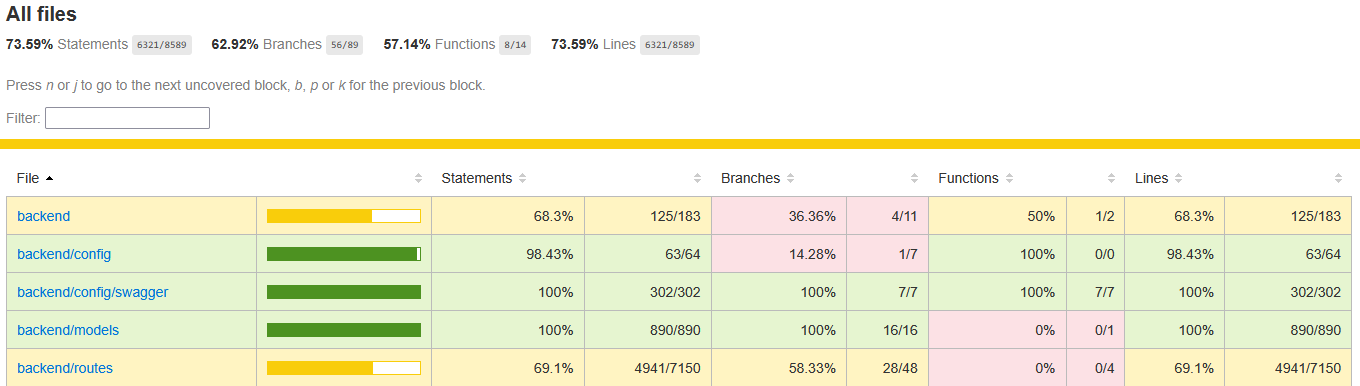
\includegraphics[width=0.8\textwidth]{cov/backend-coverage.png}
\end{center}

\subsection{Test Cases}
\begin{itemize}
    \item[\textbf{\checkmark}] \textbf{Test-Api-Info}
    \begin{itemize}
        \item \textbf{Description:} Information about our Api shows.
        \item \textbf{Reason:} To easily check if our Api is up.
    \end{itemize}
    
    \item[\textbf{\checkmark}] \textbf{Test-Public-Course-Get-Endpoint}
    \begin{itemize}
        \item \textbf{Description:} Get the all courses from public endpoint.
        \item \textbf{Reason:} Have public endpoint for external use.
    \end{itemize}
    
    \item[\textbf{\checkmark}] \textbf{Test-Private-Course-Get-Endpoint}
    \begin{itemize}
        \item \textbf{Description:} Get the all courses from private endpoint.
        \item \textbf{Reason:} Have private endpoint for getting courses.
    \end{itemize}
    
    \item[\textbf{\checkmark}] \textbf{Test-Private-Resources-Get-Endpoint}
    \begin{itemize}
        \item \textbf{Description:} Get the all resources from private endpoint.
        \item \textbf{Reason:} Have private endpoint for getting resources or specific resource.
    \end{itemize}
    
    \item[\textbf{\checkmark}] \textbf{Test-User-Get-Endpoint}
    \begin{itemize}
        \item \textbf{Description:} Check if we can get users by Id or All.
        \item \textbf{Reason:} To get all users or specific users.
    \end{itemize}
    
    \item[\textbf{\checkmark}] \textbf{Test-User-Get-notification}
    \begin{itemize}
        \item \textbf{Description:} Check if we can get users by Id or All.
        \item \textbf{Reason:} To get all users or specific users.
    \end{itemize}
    
    \item[\textbf{\sout{\ \ }}] \textbf{Authentication}
    \begin{itemize}
        \item \textbf{Description:} Testing the authentication endpoint directly.
        \item \textbf{Reason:} The test is not done because it is indirectly tested via login functionality
    \end{itemize}
\end{itemize}

\section{Frontend Tested}

\subsection{Coverage}
% Insert frontend coverage image here
\begin{center}
    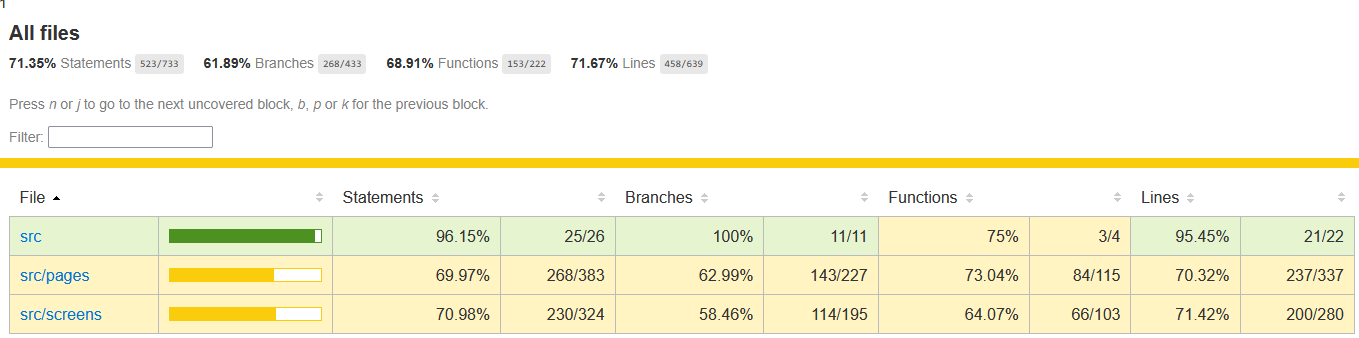
\includegraphics[width=0.8\textwidth]{cov/frontend-coverage.png}
\end{center}

\subsection{Test Cases}
\begin{itemize}
    \item[\textbf{\checkmark}] \textbf{Test-Login}
    \begin{itemize}
        \item \textbf{Description:} Test if user can correctly with Google email.
        \item \textbf{Reason:} If user cannot login they cannot use the app.
    \end{itemize}
    
    \item[\textbf{\checkmark}] \textbf{Test-Saving-State}
    \begin{itemize}
        \item \textbf{Description:} Saving the Login state for all tests to use
        \item \textbf{Reason:} To avoid being block for automated testing by Google.
    \end{itemize}
\end{itemize}

\section{Issues}

\subsection{npm Packages 2025-09-21}
\begin{itemize}
    \item 180 packages are looking for funding
    \item Run \texttt{npm fund} for details
    \item 1 low severity vulnerability
    \item To address all issues, run: \texttt{npm audit fix}
    \item Run \texttt{npm audit} for details
\end{itemize}

\subsection{Env Files Being Tracked Fix}
\begin{verbatim}
git rm --cached frontend/.env
git rm --cached frontend/.env.*
git rm --cached backend/.env
git rm --cached backend/.env.*
git commit -m "Stop tracking .env files in frontend and backend"
\end{verbatim}

\section{Package Audit Report}

\subsection{Audit Details}
\begin{itemize}
    \item \textbf{Audit Date:} 2025-09-30T13:54:43.105518
\end{itemize}

\subsection{Frontend Audit}
\begin{itemize}
    \item \textbf{Total Packages:} 584
    \item \textbf{Compromised:} 21
    \item \textbf{Compromised Percentage:} 3.6\%
    \item \textbf{Safe Percentage:} 96.4\%
\end{itemize}

\textbf{Compromised Packages:}
\begin{verbatim}
- ansi-regex@6.2.2
- ansi-styles@6.2.3
- strip-ansi@7.1.2
- wrap-ansi@8.1.0
- debug@4.1.12
- ansi-regex@5.0.1
- ansi-styles@4.3.0
- chalk@4.1.2
- color-convert@2.0.1
- color-name@1.1.4
- debug@4.4.1
- debug@4.3.7
- debug@4.3.7
- debug@1.0.0
- debug@4.3.7
- debug@4.3.7
- debug@4.3.7
- debug@4.3.7
- strip-ansi@6.0.1
- supports-color@7.2.0
- wrap-ansi@6.2.0
\end{verbatim}

\subsection{Backend Audit}
\begin{itemize}
    \item \textbf{Total Packages:} 1043
    \item \textbf{Compromised:} 34
    \item \textbf{Compromised Percentage:} 3.26\%
    \item \textbf{Safe Percentage:} 96.74\%
\end{itemize}

\textbf{Compromised Packages:}
\begin{verbatim}
- ansi-regex@6.2.2
- ansi-styles@6.2.3
- strip-ansi@7.1.2
- wrap-ansi@8.1.0
- debug@4.1.12
- ansi-regex@5.0.1
- ansi-styles@4.3.0
- debug@2.6.9
- chalk@4.1.2
- color-convert@2.0.1
- color-name@1.1.4
- debug@2.6.9
- debug@4.4.3
- debug@4.3.7
- debug@4.3.7
- error-ex@1.3.4
- debug@3.2.7
- debug@3.2.7
- debug@3.2.7
- debug@2.6.9
- debug@2.6.9
- is-arrayish@0.2.1
- supports-color@8.1.1
- debug@2.6.9
- supports-color@5.5.0
- ansi-styles@5.2.0
- debug@2.6.9
- debug@4.3.7
- debug@4.3.7
- debug@4.3.7
- debug@4.3.7
- strip-ansi@6.0.1
- supports-color@7.2.0
- wrap-ansi@7.0.0
\end{verbatim}

\subsection{Overall Summary}
\begin{itemize}
    \item \textbf{Total Packages:} 1627
    \item \textbf{Total Compromised:} 55
    \item \textbf{Overall Compromised:} 3.38\%
    \item \textbf{Overall Safe:} 96.62\%
\end{itemize}

\textbf{Assessment:} The low compromise rate (3.38\%) reflects minimal security concerns, as these vulnerabilities originate from external package dependencies rather than our core application code, presenting acceptable risk levels for our current deployment. Hance no action is required.


\chapter{Meetings Chapter}

\section{Sprint One}
% Sprint overview

\subsection{Meeting One - Planning}

\textbf{Date:} 7 August 2025 \par
\textbf{Attendees:} Backend Team \par
\textbf{Discussion:} Roles on the backend and effective communication of the structure. \par

\textbf{Minutes:}
\begin{itemize}
    \item \textbf{Roles Discussion}
    \begin{itemize}
        \item Discussed the roles that need to be shared among members. 
        \item Highlighted that one member had too many responsibilities, which hindered effective work distribution and collaboration.
        \item \textbf{Favour:} RESOURCE tables and file sharing system.
        \item \textbf{Huli:} Caching of API and group-centric tables.
        \item \textbf{Trust:} Picture-based files and backend setup.
    \end{itemize}
    
    \item \textbf{Structure}
    \begin{itemize}
        \item Emphasized the importance of core files: \texttt{models}, \texttt{index}, and \texttt{server}.
        \item Used a platform to visualize the database schema.
    \end{itemize}
    
    \item \textbf{Tasks and Objectives}
    \begin{itemize}
        \item Members need to research and become comfortable with the provided tech stack.
        \item Proper documentation required for reasoning and comparisons to alternative tools.
    \end{itemize}
\end{itemize}


\subsection{Meeting Two - Collaboration}

\textbf{Date:} 13 August 2025 \par
\textbf{Attendees:} Backend Team \par
\textbf{Discussion:} Cooperation with the independent developer team and integration of their API service. \par

\textbf{Minutes:}
\begin{itemize}
    \item \textbf{Database Updates \& Brainstorming Session}
    \begin{itemize}
        \item Discussed how to integrate a third-party application that manages events to support the organization of study sessions.
        \item Added new database tables to track information relevant to study sessions, specifically for use by group members.
    \end{itemize}
\end{itemize}


\subsection{Meeting Three - Rubric Review and Coordination}

\textbf{Date:} 16 August 2025 \par
\textbf{Attendees:} Backend \& Frontend Teams \par
\textbf{Discussion:} Review of rubric checklist and acknowledgement of successfully completed items. \par

\textbf{Minutes:}
\begin{itemize}
    \item \textbf{Task Review}
    \begin{itemize}
        \item Agreed on which tasks are considered complete and which remain incomplete.
        \item Reviewed the rubric and identified tasks to be implemented before the Sprint 1 deadline.
        \item Discussed app components that are not functioning properly.
        \item Identified actions to address the issues.
    \end{itemize}

    \item \textbf{Authentication Fault}
    \begin{itemize}
        \item Backend and frontend authentication failures were raised.
        \item Planned further debugging of server-side authentication.
    \end{itemize}

    \item \textbf{API Development Strategy}
    \begin{itemize}
        \item Agreed that all API routes will be built based on client needs, not developer assumptions.
    \end{itemize}

    \item \textbf{Branch Creation Methodology}
    \begin{itemize}
        \item Allow individual merges to the version release branch.
        \item Only approved merges to the main branch are permitted.
    \end{itemize}

    \item \textbf{LaTeX Documentation}
    \begin{itemize}
        \item All members are expected to update the shared LaTeX document on Overleaf for each feature they create.
    \end{itemize}
\end{itemize}


\subsection{Meeting Four - Rubric and LaTeX Documentation}

\textbf{Date:} 18 August 2025 \par
\textbf{Attendees:} Backend \& Frontend Teams \par
\textbf{Discussion:} Review of rubric checklist, completed items, and LaTeX documentation. \par

\textbf{Minutes:}
\begin{itemize}
    \item \textbf{LaTeX Platform}
    \begin{itemize}
        \item Each member logged in and updated the shared LaTeX file.
    \end{itemize}

    \item \textbf{Sprint 1 Rubric Review}
    \begin{itemize}
        \item Reviewed the rubric and identified required implementations that were missed for Sprint 1.
    \end{itemize}

    \item \textbf{API Requirements from Event Management Group}
    \begin{itemize}
        \item Groups table will only share \texttt{venueID}, \texttt{Name}, and \texttt{Location}.
        \item Created a separate table for the date and time of events.
    \end{itemize}

    \item \textbf{GitHub Committing}
    \begin{itemize}
        \item Implement semantic committing from now on.
    \end{itemize}
\end{itemize}


\section{Sprint Two}
% Sprint overview

\subsection{Meeting One - Backend Problem Resolution} 
\textbf{Date:} 31 August 2025 \par
\textbf{Attendees:} Backend Team \par
\textbf{Discussion:} Discussion on how the APIS work as there were problems \par

\textbf{Minutes:}
\begin{itemize}
    \item \textbf{API Dissection}
    \begin{itemize}
        \item Discussed the roles that certain APIs had within building the application. 
        \item Highlighted the fact that Using swagger to document the API was a challenge ,as a team member that had the responsibilities of a certain API, the API was not working when it was called.
        \item \textbf{Favour:} The team member with the struggle of making the API work.
        \item \textbf{Trust:} The Backend facilitator,who help with understanding the pitfalls on the API not working.
    \end{itemize}
\end{itemize}
    

\subsection{Meeting Two - Retrospective}
\textbf{Date:} 1 September 2025 \par
\textbf{Attendees:} The whole Team  \par
\textbf{Discussion:} Discussion how the sprint went and some resolutions for the following sprints \par

\textbf{Minutes:}
\begin{itemize}
    \item \textbf{API Dissection}
    \begin{itemize}
        \item Discussed the problematic integration of the API with the frontend as some were not working for days and it hindered progress. 
        \item Discussed the impact that us not having meetings was a problem as some team members were working blindly and there was no communication that was solid except on whatsApp when a problem arouse we solved it through text and this limited productivity.
        \item \textbf{Resolutions:} The team members all agreed to try and improve the amount of times we meet and have a fixed schedule for meetings that will not change unless there is an emergency.Smaller meetings to be had with backend team if there is an issue with the backend and not involving the frontend team as this will waste time.Team Discussed the importance of reading messages that are communicated on whatsApp thoroughly as they may contain intel and minimise confusion.
        \item \textbf{Reasons of Problems:}The team didnt meet as a result of this week being hectic with regards to submissions and there being a test written that needed undivided attention.This truly messed up the teams productivity in balancing and finishing the work in a timely manner.Some days were reserved as some team members have religious practices like the saddath day as well as bible study to uphold,these could have been used to push work thoroughly.
    \end{itemize}
\end{itemize}

\section{Sprint Three}
% Sprint overview

\subsection{Meeting One - Planning}
% Planning meeting details

\subsection{Meeting Two - Retrospective}
% Retrospective outcomes

\section{Sprint Four}
% Sprint overview

\subsection{Meeting One - Planning}
%Planning meeting details

\subsection{Meeting Two - Final Retrospective}
% Final retrospective outcomes

\chapter{Pitfall Chapter}

Your chapter content goes here. 

\section{First Section}
% example content, replace with your real content

\subsection{A Subsection}


% Pitfall 1
\subsubsection*{Pitfall: Documentation}
\textbf{Description:} During development, we documented things but not in order that makes sense and we left out a lot of things that were truly important.  

\textbf{Resolution:} Each member was instructed that when documenting on Papeeria to ensure that errors are mitigated immediately and not left for other people to solve.  

% Pitfall 2
\subsubsection*{Pitfall: API connection to Frontend}
\textbf{Description:} There were multiple APIs that were built and not working so when the Frontend needed them they found out that they were not working,hence curbing productivity this is also as a result of the Backend having multiple issues.  

\textbf{Resolution:} Had small meeting with the Backend to ensure smooth running APIs as well as agreed that they should be tested before the Frontend team uses them.

% Pitfall 3
\subsubsection*{Pitfall: External API not ready}
\textbf{Description:} Initially we had a team building the Event management application that agreed to integrate their API with our team after some days they reached out and informed us that they cannot provide the API we need so that we can integrate our application.  

\textbf{Resolution:} The team will continue to look for alternative teams that can integrate our API with our application or change the way in which we need the API incase we do not in a timely manner.
\chapter{User Feedback}

\section{Overview}
This chapter presents feedback from users who interacted with Study Buddy.  
It highlights the users, experiences, perceptions, and suggestions.  
The goal is to understand how the application performs in real scenarios, what users like, and areas for improvement.

\section{Purpose of the Chapter}
The purpose of this chapter is to:
\begin{itemize}
    \item Summarize user experiences.
    \item Identify strengths and weaknesses of Study Buddy.
    \item Provide actionable insights for future improvements.
\end{itemize}

\section{User Feedback Responses}

\subsection*{User 1: Brilliant Mukgwedi}
\begin{itemize}
    \item Likely usage: Daily
    \item Main purpose: Accessing or sharing resources
    \item Rating: 2 stars
    \item Ease of navigation: Difficult
    \item Most useful feature: Resource sharing
    \item Satisfaction with group discussions and private messages: Not satisfied
    \item Comments: Likes the website for educational purposes and obtaining resources for courses. Suggested adding more features to make it holistic.
\end{itemize}

\subsection*{User 2: Lufuno Tshifhiwa}
\begin{itemize}
    \item Likely usage: Several times a week
    \item Main purpose: Accessing or sharing resources
    \item Rating: 5 stars
    \item Ease of navigation: Very easy
    \item Most useful features: Resource sharing, connecting with new people
    \item Satisfaction with group discussions and private messages: Very satisfied
    \item Comments: Likes the ease of use of the website.
\end{itemize}

\subsection*{User 3: Devine Onwenu}
\begin{itemize}
    \item Likely usage: Occasionally
    \item Main purpose: Accessing or sharing resources
    \item Rating: 3 stars
    \item Ease of navigation: Easy
    \item Most useful feature: Connecting with new people
    \item Satisfaction with group discussions and private messages: Neutral
    \item Comments: Likes the simplicity of the website and suggested improvements for accessibility.
\end{itemize}

\subsection*{User 4: Maybe Kgaugelo}
\begin{itemize}
    \item Likely usage: Occasionally
    \item Main purpose: Group discussions
    \item Rating: 5 stars
    \item Ease of navigation: Easy
    \item Most useful feature: Group discussions
    \item Satisfaction with group discussions and private messages: Satisfied
    \item Comments: Enjoys group discussions with friends.
\end{itemize}

\subsection*{User 5: Malebo Munyai}
\begin{itemize}
    \item Likely usage: Several times a week
    \item Main purpose: Sharing insights and knowledge
    \item Rating: 4 stars
    \item Ease of navigation: Easy
    \item Most useful features: Group discussions, Resource sharing
    \item Satisfaction with group discussions and private messages: Satisfied
    \item Comments: Likes the ease of navigation on the website.
\end{itemize}

\subsection*{User 6: Thabiso Mofokeng}
\begin{itemize}
    \item Likely usage: Daily
    \item Main purpose: Accessing or sharing resources
    \item Rating: 4 stars
    \item Ease of navigation: Neutral
    \item Most useful features: Group discussions, Resource sharing
    \item Satisfaction with group discussions and private messages: Neutral
    \item Comments: Likes the ability to share resources.
\end{itemize}

\subsection*{User II: Daniel}
\begin{itemize}
    \item Comments: Mentioned the application was fast and efficient. Suggested adding a walkthrough/tutorial for first-time users to explain buttons and pages.
\end{itemize}

\subsection*{User III: Khanyisile Ndlovu}
\begin{itemize}
    \item Comments: Liked the notifications feature and linked course recommendations. Requested more customization options.
\end{itemize}

\subsection*{User IV: Thato Shandu}
\begin{itemize}
    \item Comments: Found the application visually appealing. Suggested improving feedback forms to be more user-friendly and requested a holistic view of the full application.
\end{itemize}

\subsection*{User V: Simphiwe Mathe}
\begin{itemize}
    \item Comments: Praised the stability of the application. Recommended adding an FAQ or help section for new users.
\end{itemize}

\section{Summary of Suggested Improvements}
Based on the collected feedback, several areas for improvement and additional features have been identified. Key observations include:

\begin{itemize}
    \item Users appreciated the intuitive interface, responsiveness, and stability.
    \item There is a need for guidance for first-time users, including tutorials or walkthroughs.
    \item Feedback forms should be improved to be more user-friendly.
    \item Users requested more customization options for notifications and course recommendations.
    \item Adding an FAQ or help section would assist new users.
\end{itemize}

This feedback was collected by sharing the deployed application link with friends and colleagues, allowing them to interact with the live system and provide honest opinions.

\section{Improvements made to accomodate users}
\begin{itemize}
    \item Implemented more features such as adding a friend recommendations, comment sections, group activities etc...
    \item Made some improvements with the look and feel for private chats.
    \item We aim to continue with adding more features and improvements for group discussions in the future sprint.
    \item We improved the websites response time for both mobile and computers to improve user experience and usability.
    \item Made changes to the user feedback forum to be more pleasing to the eye and intuitive to use.
\end{itemize}

\section{Link to Google Form User Feedbacks}
For reference and further responses, the Google Form can be accessed here: \\
\url{https://forms.gle/VkPyoACzZmBmYbd57}

\chapter{Database Documentation}

\section{Database Setup}

\subsection{Option A: Local PostgreSQL}
\begin{enumerate}
    \item Install PostgreSQL locally.
    \item Create a database.
    \item Update the \texttt{.env} file with your local credentials.
\end{enumerate}

\subsection{Option B: NeonDB (Recommended)}
\begin{enumerate}
    \item Sign up at \url{https://neon.tech}.
    \item Create a new project.
    \item Copy the connection string.
    \item Update the \texttt{.env} file with NeonDB credentials.
\end{enumerate}

\section{Database Operations}

\begin{lstlisting}[language=bash, caption=Database Commands]
# Run migrations
npm run db:migrate

# Seed database
npm run db:seed

# Reset database
npm run db:reset
\end{lstlisting}

\section{Database Configuration}

\subsection{Sequelize Setup}
The application uses Sequelize ORM with PostgreSQL for database interaction. 
Key configuration is stored in \texttt{config/database.js}:

\begin{lstlisting}[language=JavaScript, caption=Sequelize Configuration]
const sequelize = new Sequelize(
  process.env.DB_NAME,
  process.env.DB_USER,
  process.env.DB_PASSWORD,
  {
    host: process.env.DB_HOST,
    port: process.env.DB_PORT,
    dialect: 'postgres',
    logging: process.env.NODE_ENV === 'development',
    dialectOptions: {
      ssl: {
        require: true,
        rejectUnauthorized: false
      }
    }
  }
);
\end{lstlisting}

\subsection{Models}
\begin{itemize}
    \item \textbf{User:} Stores authentication and profile data.
    \item Easily extensible for additional models as required.
\end{itemize}

\section{Development Workflow}

\subsection{Starting Development}
\begin{lstlisting}[language=bash]
# Install dependencies
npm install

# Set up environment
cp env.example .env
# Edit .env with your database credentials

# Start development server
npm run dev
\end{lstlisting}

\subsection{Database Changes}
\begin{lstlisting}[language=bash]
# Enable database sync for development
ENABLE_DB_SYNC=true

# Use migrations for production
npm run db:migrate
\end{lstlisting}

\subsection{Testing APIs}
\begin{itemize}
    \item Visit \url{http://localhost:3000/api-docs} for interactive documentation.
    \item Use Postman or curl for API testing.
\end{itemize}

\section{Production Deployment}

\subsection{Environment Setup}
\begin{lstlisting}[language=bash]
NODE_ENV=production
ENABLE_DB_SYNC=false  # Never sync in production
\end{lstlisting}

\subsection{Security Considerations}
\begin{itemize}
    \item Change all default secrets.
    \item Use strong JWT secrets.
    \item Enable HTTPS.
    \item Configure proper CORS origins.
    \item Set up rate limiting.
\end{itemize}

\subsection{Database}
\begin{itemize}
    \item Use production-grade PostgreSQL.
    \item Set up automated backups.
    \item Configure connection pooling.
    \item Always use migrations instead of sync.
\end{itemize}

\section{Troubleshooting}

\subsection{Common Issues}
\begin{description}
    \item[Database Connection Failed:] Verify \texttt{.env} credentials and network connectivity.
    \item[Port Already in Use:] Change the port or use \texttt{npx kill-port 3000}.
    \item[Module Not Found:] Run \texttt{npm install} and check Node.js version.
    \item[Database Sync Issues:] Set \texttt{ENABLE\_DB\_SYNC=true} for development; use migrations for production.
\end{description}

\subsection{Logs}
\begin{itemize}
    \item Application logs appear in the console.
    \item Database queries are logged in development mode.
    \item Error details are displayed in development mode.
\end{itemize}

\section{Scripts Reference}
\begin{lstlisting}[language=json, caption=Package Scripts]
{
  "start": "node server.js",
  "dev": "nodemon server.js",
  "test": "jest",
  "db:migrate": "sequelize-cli db:migrate",
  "db:seed": "sequelize-cli db:seed:all",
  "db:reset": "sequelize-cli db:drop && sequelize-cli db:create && sequelize-cli db:migrate && sequelize-cli db:seed:all"
}
\end{lstlisting}

\section{Next Steps}
\begin{itemize}
    \item Add more models as required.
    \item Implement unit and integration tests.
    \item Introduce structured logging.
    \item Add health checks and monitoring.
    \item Set up a CI/CD pipeline for automated deployments.
\end{itemize}

\section{Support}
\begin{itemize}
    \item Refer to the troubleshooting section for common issues.
    \item Review API documentation at \url{/api-docs}.
    \item Check console logs for error details.
    \item Ensure all environment variables are correctly set.
\end{itemize}


\section{Database Schema}

This section describes the schema used to store application data. Below is an example of the \texttt{notifications} table schema from our Neon database instance.

\subsection{Notifications Table}

\begin{table}[H]
\centering
\begin{tabular}{|l|l|l|l|}
\hline
\textbf{Column} & \textbf{Data Type} & \textbf{Constraints} & \textbf{Description} \\
\hline
\texttt{id} & SERIAL & PRIMARY KEY & Unique identifier for each notification. \\
\hline
\texttt{user\_id} & UUID & NOT NULL & References the user receiving the notification. \\
\hline
\texttt{message} & VARCHAR(255) & NOT NULL & The content of the notification. \\
\hline
\texttt{title} & VARCHAR(255) & NOT NULL & Title or subject of the notification. \\
\hline
\texttt{read} & BOOLEAN & NOT NULL, DEFAULT FALSE & Indicates if the notification has been read. \\
\hline
\texttt{created\_at} & TIMESTAMP WITH TIME ZONE & NOT NULL & Timestamp when the notification was created. \\
\hline
\end{tabular}
\caption{Schema for the \texttt{notifications} table.}
\end{table}




\section{Choice Justification}

In selecting a database solution for this project, Neon DB emerged as the most effective and forward-thinking option, surpassing traditional relational databases in flexibility, scalability, and performance. Neon offers a fully managed, serverless PostgreSQL platform, meaning it provides all the robust relational features of PostgreSQL while introducing modern cloud-native benefits such as autoscaling, high availability, and instant branching for development and testing. 

Our project required a solution that could elegantly handle relational data, linking entities such as users, resources, and reports without compromising speed or reliability. Neon was the ideal fit because it allowed us to seamlessly model relationships between tables while benefiting from PostgreSQL’s mature query capabilities. Unlike many other databases that either limit relational functionality (as seen in certain NoSQL systems) or impose heavy maintenance overhead (as with self-hosted relational databases), Neon combines ease of use with enterprise-grade reliability. 

Additionally, Neon’s separation of compute and storage makes scaling cost-efficient and straightforward, ensuring that our application can evolve without disruptive migrations or manual scaling efforts. Its seamless integration with ORMs like Sequelize further streamlines development, allowing our team to maintain a clean codebase while interacting with the database intuitively. This strategic choice ensures that we can confidently build a future-proof application with high performance, robust data integrity, and operational simplicity.


\section{High End Overview}

\begin{itemize}
    \item \textbf{User-Centric Relationships}: 
    \begin{itemize}
        \item The \texttt{User} table is central; most tables reference it via \texttt{user\_id}, establishing clear ownership.
        \item Tables like \texttt{Notifications}, \texttt{PrivateChats}, \texttt{Progress}, and \texttt{Study\_sessions} are one-to-many with \texttt{User}.
    \end{itemize}

    \item \textbf{Many-to-Many Relationships}:
    \begin{itemize}
        \item \texttt{UserCourses} links \texttt{Users} and \texttt{Courses}.
        \item \texttt{Group\_members} links \texttt{Users} and \texttt{Study\_groups}.
        \item \texttt{Likes} links \texttt{Users} and \texttt{Resources}.
        \item These join tables avoid data duplication but can grow large with many users or resources.
    \end{itemize}

    \item \textbf{Self-Referencing Relationships}:
    \begin{itemize}
        \item \texttt{Follows} and \texttt{Follows\_requests} implement social connections between users.
        \item Requires careful indexing to maintain query performance as the user count grows.
    \end{itemize}

    \item \textbf{Resource-Centric Relationships}:
    \begin{itemize}
        \item \texttt{Resources} connect to \texttt{Resource\_tags}, \texttt{Resource\_threads}, and \texttt{Resource\_reports}.
        \item High-traffic resources may create join hotspots.
    \end{itemize}
    
     \item \textbf{Structure observation}:
    \begin{itemize}
        \item \textbf{Normalisation}--- our data is clearly normalised as a result of non redundant data each piece of information is stored only once (e.g., UserCourses links Users and Courses instead of repeating course info for every user).Separate tables for entities-  Users, Courses, Resources, Likes, Groups, etc., each have their own table.
        \item Foreign keys instead of repeated data – Relationships are handled via foreign keys (user\_id, course\_id, etc.) rather than duplicating user or course details.
    \end{itemize}

    \item \textbf{Scalability Considerations}:
    \begin{itemize}
        \item Proper indexing on foreign keys is essential (\texttt{user\_id}, \texttt{resource\_id}, \texttt{course\_id}, etc.).
        \item Many-to-many relationships scale quadratically, with active users and resources.
        \item Database scalability is addressed with indexing, query optimization, caching (e.g., Redis).
    \end{itemize}
\end{itemize}

\chapter{API Integration}
\label{chap:apiintegration}

In this chapter, we discuss the integration of third-party Application Programming Interfaces (APIs) that enhance the functionality, scalability, and security of our system. Specifically, we focus on the use of the \textbf{Google Authentication API} and the \textbf{Firebase Authentication API}. These APIs were chosen due to their robust features, ease of integration, and ability to provide secure, reliable user authentication.

\section{Google Authentication API}
The Google Authentication API (Google Auth) enables users to log in using their existing Google accounts, reducing friction during registration and ensuring a seamless onboarding process. By leveraging OAuth 2.0 and OpenID Connect, Google Auth ensures:
\begin{itemize}
    \item \textbf{Enhanced Security:} OAuth 2.0 provides token-based authentication, which eliminates the need to handle user passwords directly, reducing vulnerability to data breaches.
    \item \textbf{User Convenience:} Users can sign in without creating a new username and password, improving accessibility and reducing account management overhead.
    \item \textbf{Scalability:} The integration scales efficiently to accommodate a growing user base, as the authentication process is managed by Google’s reliable infrastructure.
    \item \textbf{Cross-Platform Support:} Google Auth works across multiple devices and platforms, ensuring consistent login experiences for users.
\end{itemize}

\section{Firebase Authentication API}
Firebase Authentication complements Google Auth by offering a comprehensive, developer-friendly authentication solution that supports multiple sign-in methods, including email/password, phone number verification, and third-party identity providers.
\begin{itemize}
    \item \textbf{Ease of Implementation:} Firebase provides Software Development Kits (SDKs) for popular programming languages and frameworks, reducing development complexity.
    \item \textbf{Real-Time Sync:} As part of the Firebase ecosystem, authentication status can be synchronized in real-time with other Firebase services, such as Firestore or Realtime Database.
    \item \textbf{Secure Token Management:} Firebase automatically handles token generation, renewal, and expiration, ensuring high levels of security.
    \item \textbf{Customizable User Experience:} Firebase offers customizable authentication flows to align with the branding and design of the application.
\end{itemize}

\section{Justification of API Choices}
The decision to integrate Google Auth and Firebase Authentication was driven by the need to provide a secure, scalable, and user-friendly authentication mechanism. Using these APIs offers the following advantages:
\begin{enumerate}
    \item \textbf{Security Best Practices:} Both APIs use industry-standard encryption and authentication protocols, reducing risks associated with password storage.
    \item \textbf{Reduced Development Overhead:} Leveraging these mature APIs significantly decreases the time and resources required to implement and maintain authentication features.
    \item \textbf{Reliability and Scalability:} Both Google and Firebase are backed by Google Cloud’s infrastructure, ensuring minimal downtime and high scalability for future growth.
    \item \textbf{Integration Flexibility:} These APIs integrate seamlessly with various frontend frameworks, backend services, and cloud environments, allowing for a flexible system design.
\end{enumerate}


\section{Event App API integration:}
The team has been fortunate to find a group that will lend us their deployed api,regarding the events ,we plan to use their api in such a way that we can use their events that they created as a way in which Study buddy users can make an event that will correlate to study session.
\begin{enumerate}
    \item \textbf{Concerns:} We can create an event according to their schema but we ran through the issue of how we will access it to display on our application.
    \item \textbf{Discussed on parsing their api to backend:} The team came out with a viable strategy to use their API by asking for additional information on how to better use their api as asking them to change their api would be not ideal.
    \url {https://codexa-v1.github.io/Codexa/development/BackendApi.html}
\end{enumerate}

\section{Google Calender API:}
The team has agreed to integrate study buddy with google calender API ,reason being is that students can mount studdy session events on it and it could be synced to any device as long as they have google.
\begin{enumerate}
    \item \textbf{Concerns:} Pricing ,will we need to change some endpoints to make it a suitable add on.
\end{enumerate}


\section{Study Buddy API-scrutiny}
This section evaluates the architecture, robustness, and scalability measures implemented in the Study Buddy API. It highlights the testing approach, schema design, scalability considerations, and deployment practices.

\begin{enumerate}
    \item \textbf{Stress Testing:} 
    The API undergoes regular stress and load testing to evaluate its performance under high-traffic scenarios. Postman Runner is used to simulate concurrent users and heavy request loads. Metrics such as response time, throughput, and error rate are measured to identify bottlenecks and improve system resilience.

    \item \textbf{Schema Robustness:} 
    The API follows a well-defined RESTful schema with clear API naming conventions according to endpoints use (e.g., \texttt{/users/123}). Proper use of HTTP status codes and versioning strategies further improves reliability and forward compatibility.

    \item \textbf{Scalability Measures:} 
    The API is designed to be stateless, meaning each request contains all necessary context (e.g., authentication via JWT). This enables horizontal scaling by distributing traffic across multiple servers using load balancers. Rate limiting and throttling mechanisms are in place to prevent abuse and maintain service quality.

    \item \textbf{Deployed Site Practices:} 
    The api is deployed on Render platform,as Render lets you provision PostgreSQL databases, run cron jobs, and set up background workers alongside your API — all within one dashboard.
    \item \url{https://sdp-project-zilb.onrender.com}
\end{enumerate}


Overall, the integration of these APIs improves the system’s authentication capabilities, enabling developers to focus more on core features while ensuring user data security and a smooth user experience.


\chapter{Wireframes}


Wireframes are essential for visualizing the layout and structure of an application before implementation. 
The following figures illustrate the wireframe designs for the application’s key screens.

\begin{figure}[htbp] % Placement options: h=here, t=top, b=bottom, p=page
    \centering
    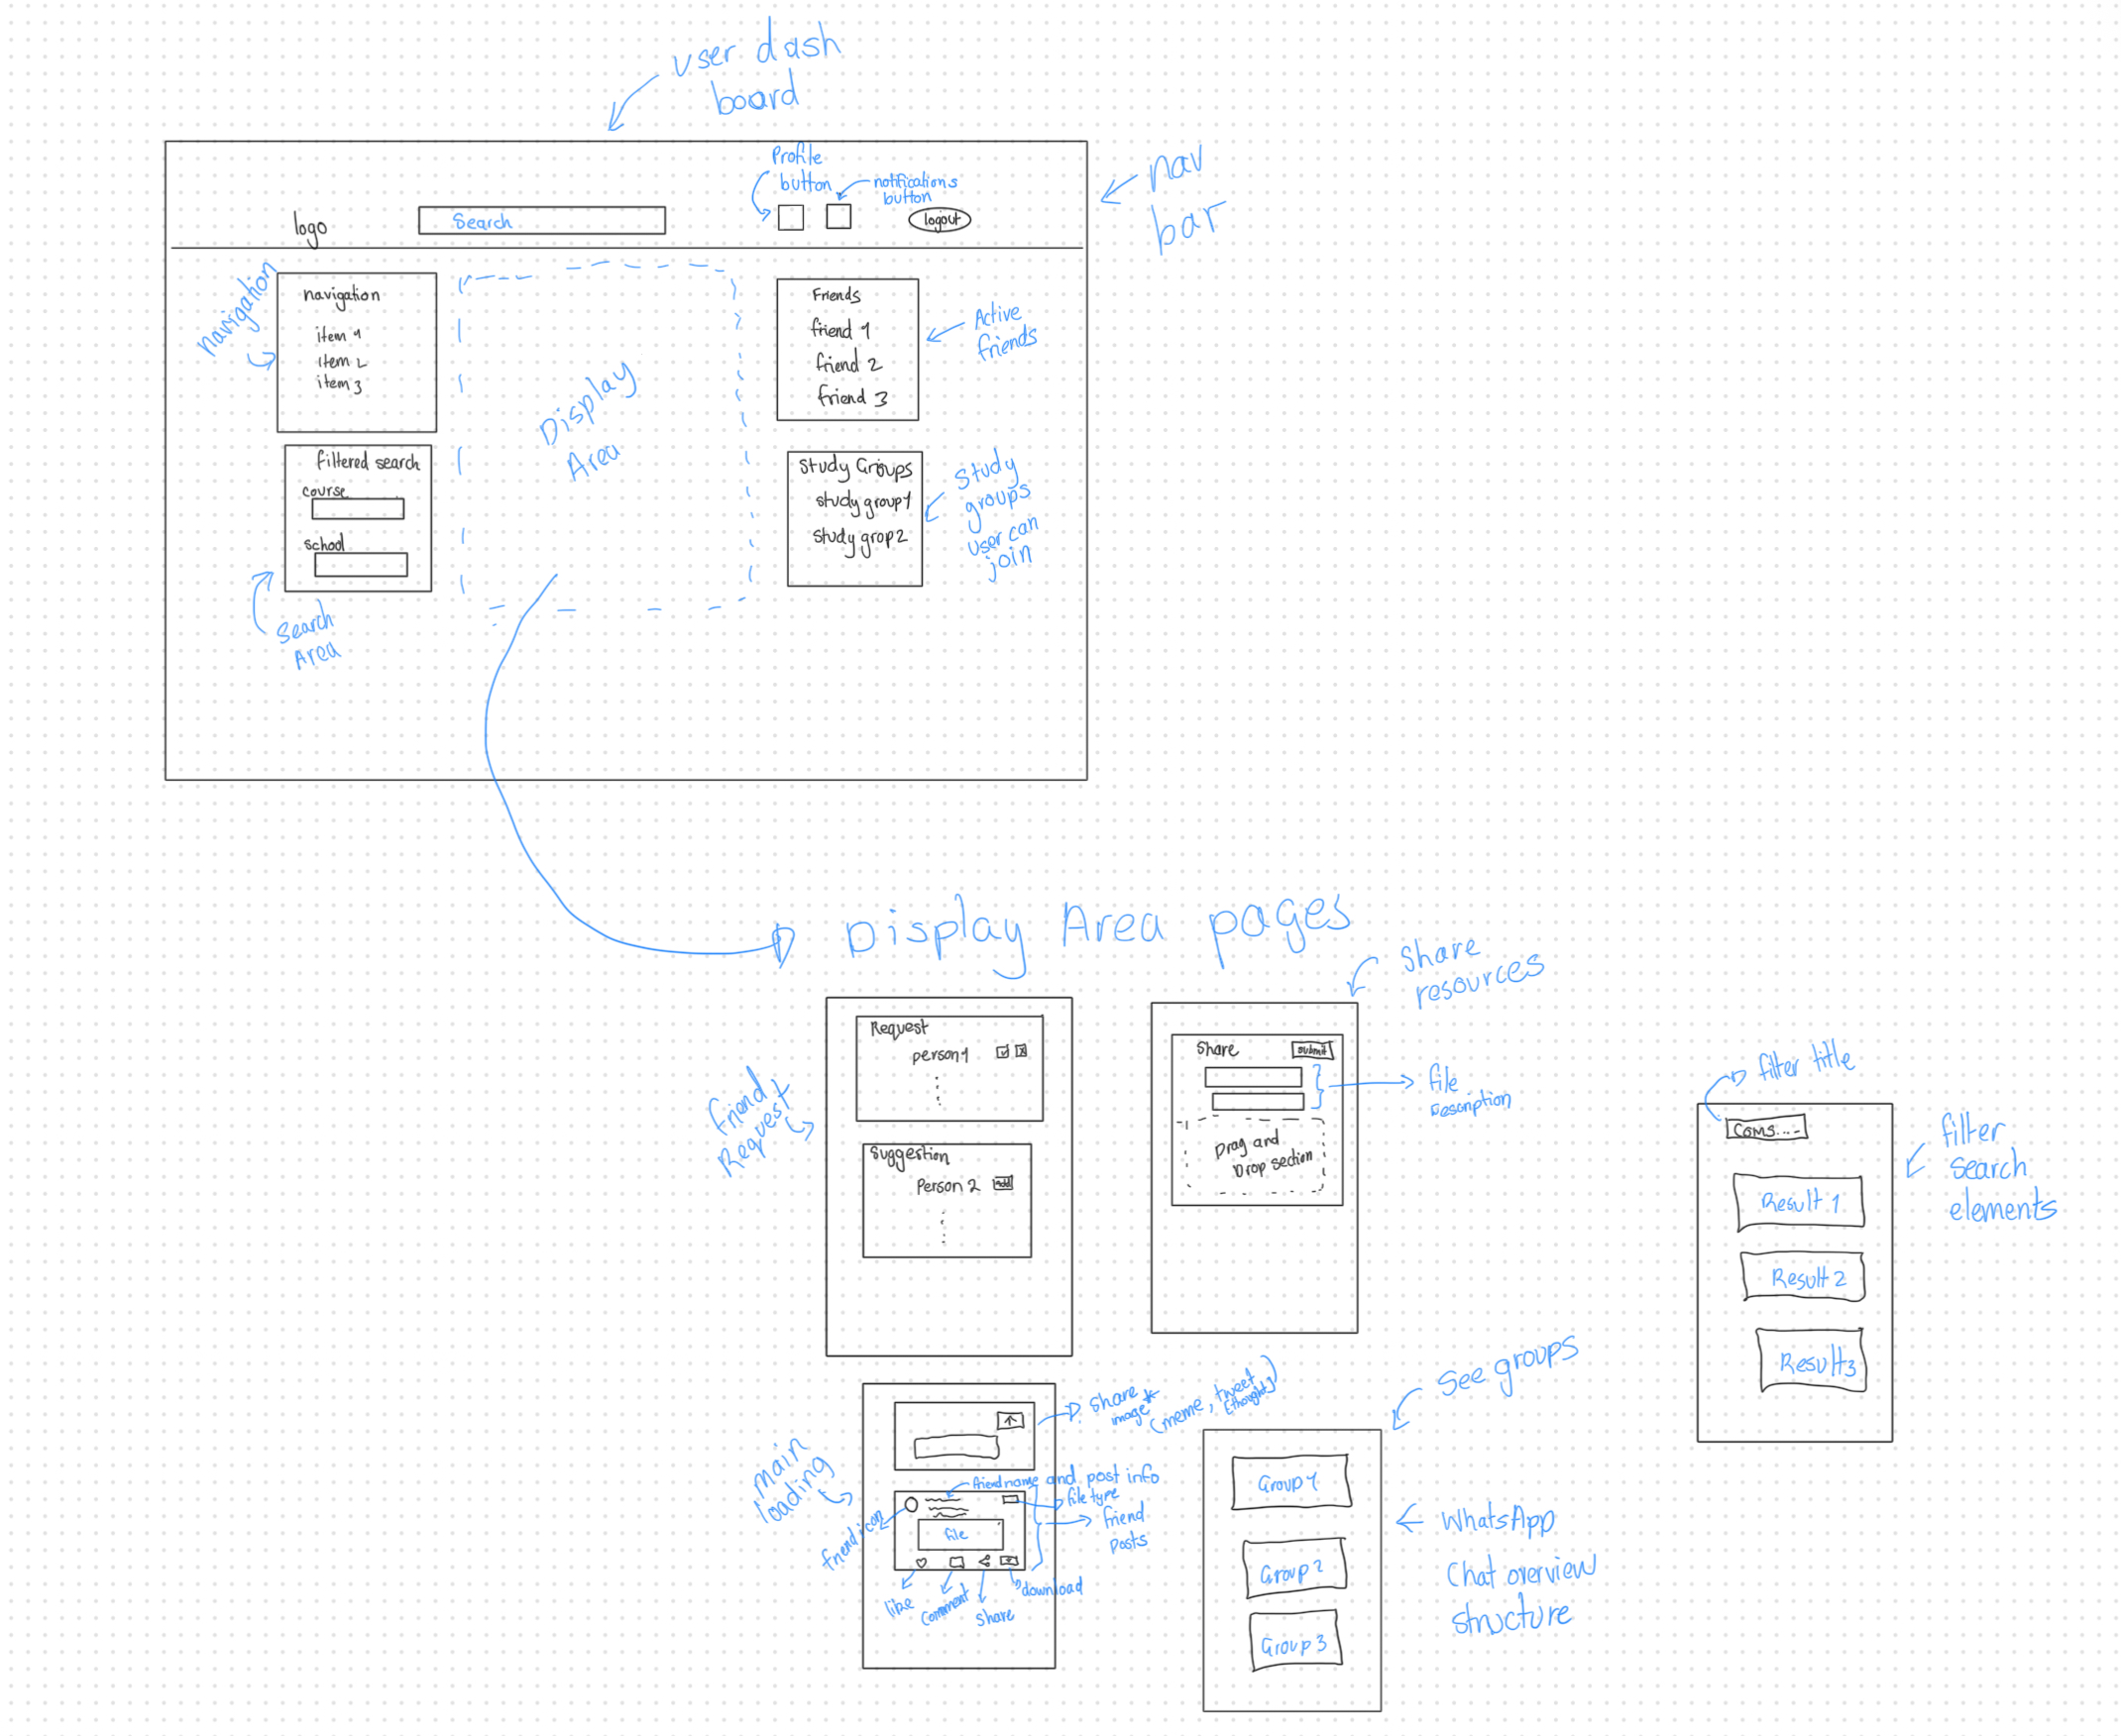
\includegraphics[width=0.8\textwidth]{IMG_3186.jpg}
    \caption{Dashboard UI}
    \label{fig:wireframe1}
\end{figure}



\section*{Discussion}
These wireframes provide a blueprint for the user interface, ensuring consistency and usability throughout the application.

\chapter{Features}

\begin{itemize}

    \item \textbf{Power feat:Resources} 
    \begin{itemize}
        \item Can be able to add resources pdfs and images.
        \item Resources can be liked as well as commented on adding the feature of other users to have more intel if a certain Resource has been beneficial to their studying.
        \item Can be able to search resources by title.
        \item Can be able to download resources and save them locally.
        \item Implemented this feature as resources being shared are important as they help students to study materials that are related to their course without wasting time looking at a myriad of things that are not related at all to their current study period
        \item Resources that are shared by friends are what can be seen so we do not expect users to see all the resources that are uploaded into the application .Only people that are accepted as friend requests are the only peoples resources that you can see.
    \end{itemize}
    
    \item \textbf{Find Study buddies} 
    \begin{itemize}
        \item View profiles of people using the study Buddy application by clicking their names on dashboard.
        \item Can be able to see all the interests of the other student,as you view their profile.
        \item Makes suggestions and can be able to accept friends request from people using the application.
        \item With wanting to make a friend ,users can go to the study buddy navigation and can press the add add friend so that people could be added as friends .Then the above functionalities will  apply as friend requests have been established.
    \end{itemize}

    \item \textbf{Create Study Groups} 
    \begin{itemize}
        \item Create,leave and join group study groups .
        \item Within my groups functionality  you can see the groups you are in as well as have the ability to create sessions where by time and location can be inserted so that members know the specific details of these. 
        \item Implemented real-time chat system where clicking a persons profile ensures the chat system appears and can be ready for use .
        \item Chat system has real-time message retrieval system.
    \end{itemize}

    \item \textbf{Track Your Progress} 
    \begin{itemize}
        \item Calendar event planner ,when click on date it will show you the reminder and time to finish that task
        \item Log any completed topics, subtopics, and sections .
        \item Track and view hours spent studying.
        \item Can be able to see study sessions that were planned according to the study groups that you are in.
    \end{itemize}

    \item \textbf{Plan Sessions} 
    \begin{itemize}
        \item Notifications are done theres a notifications page that appears with all the notifications about tasks .
        \item Add automatic reminder through email -- in progress
        \item Schedule future study sessions with reminders within study groups .
    \end{itemize}
\end{itemize}

\chapter{Stakeholder}

\begin{itemize}

    \item \textbf{Email sign in} 
    \begin{itemize}
        \item Client proposed that we add a feature to sign in to the application through email and password ,adding upon the gmail(google sign in).
        \item Done - implemented this through firebase as we dont want to be responsible for storing personal user information like passwords and emails as its risky.
        \item \textbf{Status} -- Done.
    \end{itemize}

    \item \textbf{Google Calendar API} 
    \begin{itemize}
        \item Client got engaged and recommended the integration of google calendar api as they saw how it could be well suited to store study events for students.
        \item Cost was the concern our client highlighted as something to lookout for.
        \item \textbf{Status} -- Done.
    \end{itemize}

    \item \textbf{Comment section under resources} 
    \begin{itemize}
        \item Client found this fascinating and liked the idea behind this feature as well as the liking of resources.
        \item \textbf{Status} -- Done.
    \end{itemize}
    
    \item \textbf{Enhancing the Friend request UI} 
    \begin{itemize}
        \item Client adviced the team to add better ui elements to the friends list instead of the blank letters of the user name hence improving usability and improving aesthetic feel.
        \item \textbf{Status} -- Done.
    \end{itemize}

    \item \textbf{feat: filter resources by friends instead of all} 
    \begin{itemize}
        \item The Client mentioned the fact that users should see resources that are posted by their friends instead of making it broad and seeing all resources as it could overwhelm the student.
        \item \textbf{Status} -- In progress.
    \end{itemize}
    
    \item \textbf{Group features} 
    \begin{itemize}
        \item Client liked the idea of having groups that he can join freely and interact with the people who are also the member of the group.
        \item \textbf{Status} -- Done.
    \end{itemize}
    
\end{itemize}

\chapter{Performance}

\section{Google Lighthouse}

Google Lighthouse is an open-source, automated tool developed by Google to improve the quality of web pages. It provides audits for performance, accessibility, best practices, SEO, and progressive web apps. By running Lighthouse, developers receive detailed reports with actionable recommendations to optimize their websites. The main benefits include faster page load times, improved user experience, better accessibility compliance, enhanced search engine visibility, and adherence to modern web standards. Lighthouse can be run in Chrome DevTools, from the command line, or integrated into continuous integration pipelines to ensure consistent web performance improvements.

\section{Mobile}

\textbf{Metrics:}
\begin{itemize}
    \item First Contentful Paint - 1.7s
    \item Total Blocking Time - 20ms
    \item Speed Index - 1.7s
    \item Largest Contentful Paint - 4.4s
    \item Cumulative Layout Shift - 0.111
\end{itemize}

\begin{figure}[H] % Forces figure here
    \centering
    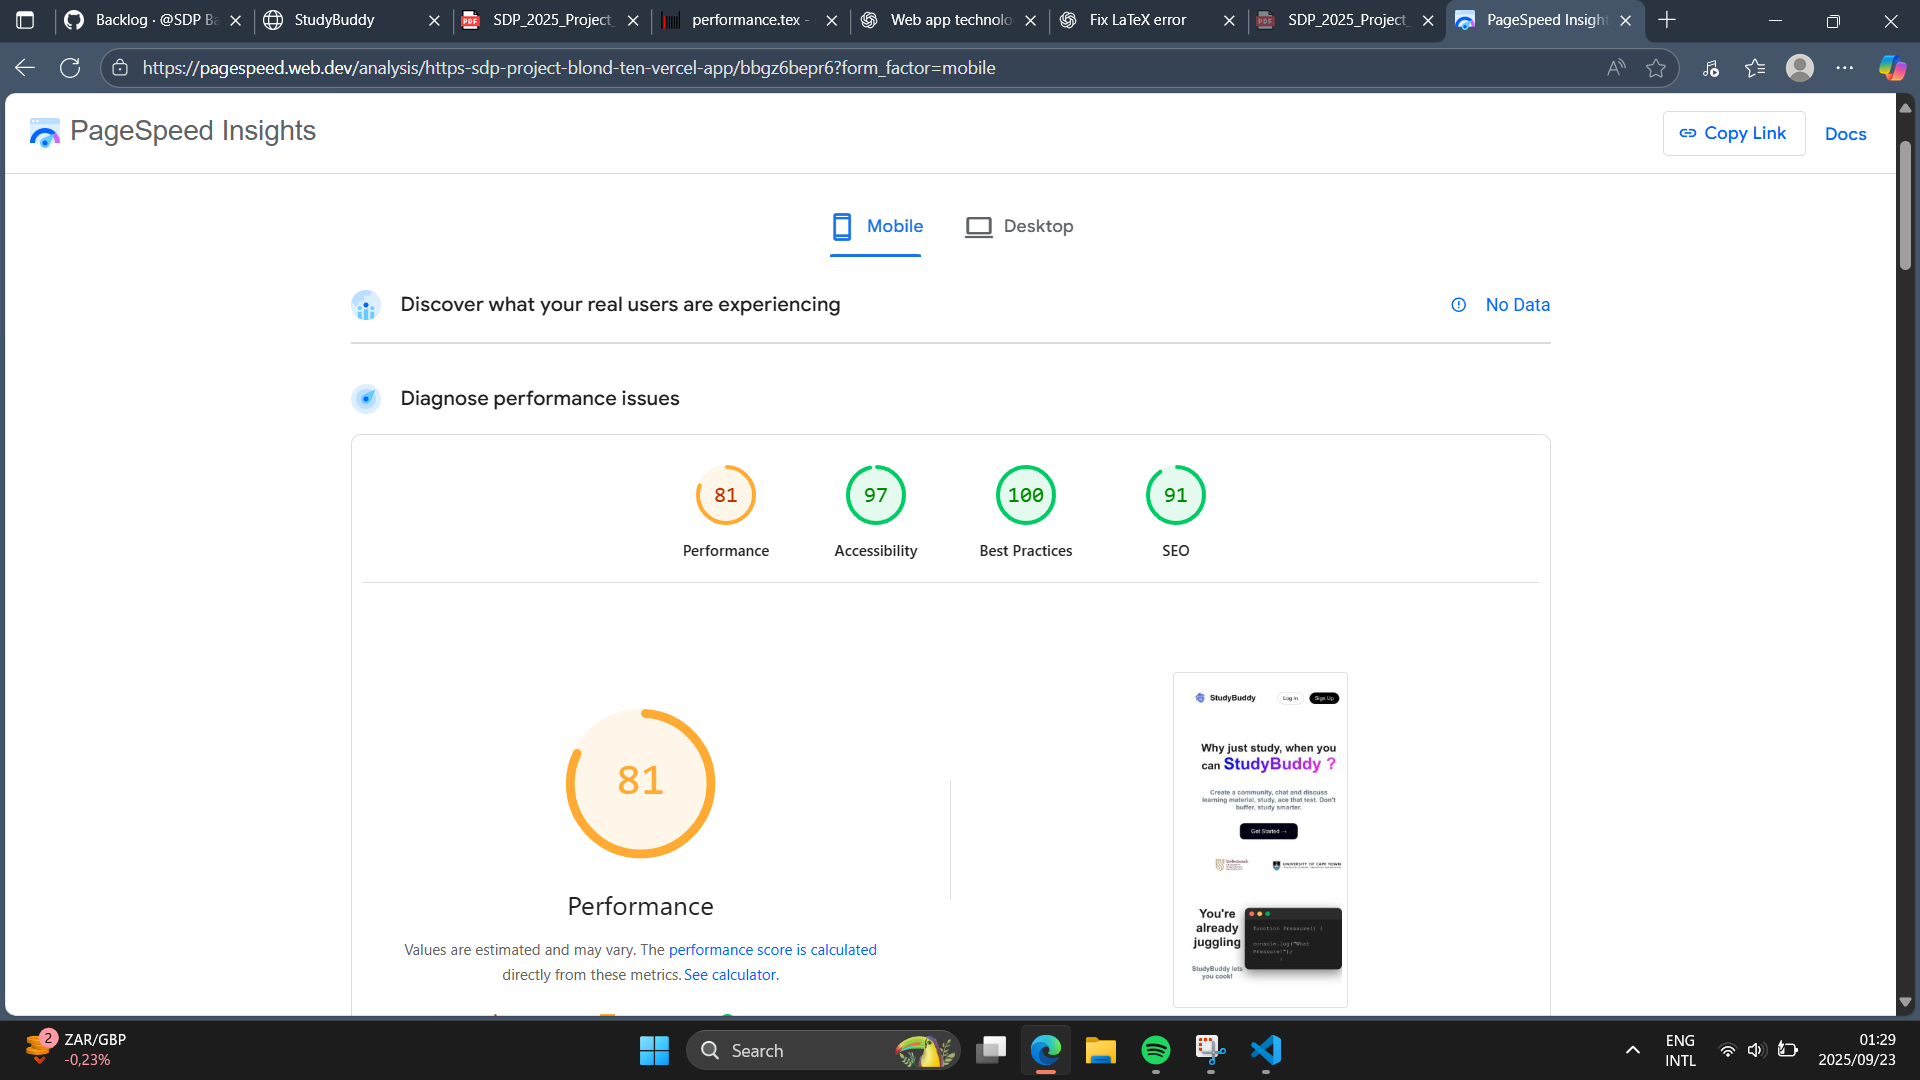
\includegraphics[width=0.8\textwidth]{mobile.png}
    \caption{How Study Buddy performs on mobile devices}
    \label{fig:mobile_performance}
\end{figure}

\section{Desktop}

\textbf{Metrics:}
\begin{itemize}
    \item First Contentful Paint - 0.4s
    \item Total Blocking Time - 0ms
    \item Speed Index - 0.4s
    \item Largest Contentful Paint - 0.8s
    \item Cumulative Layout Shift - 0.118
\end{itemize}

\begin{figure}[H]
    \centering
    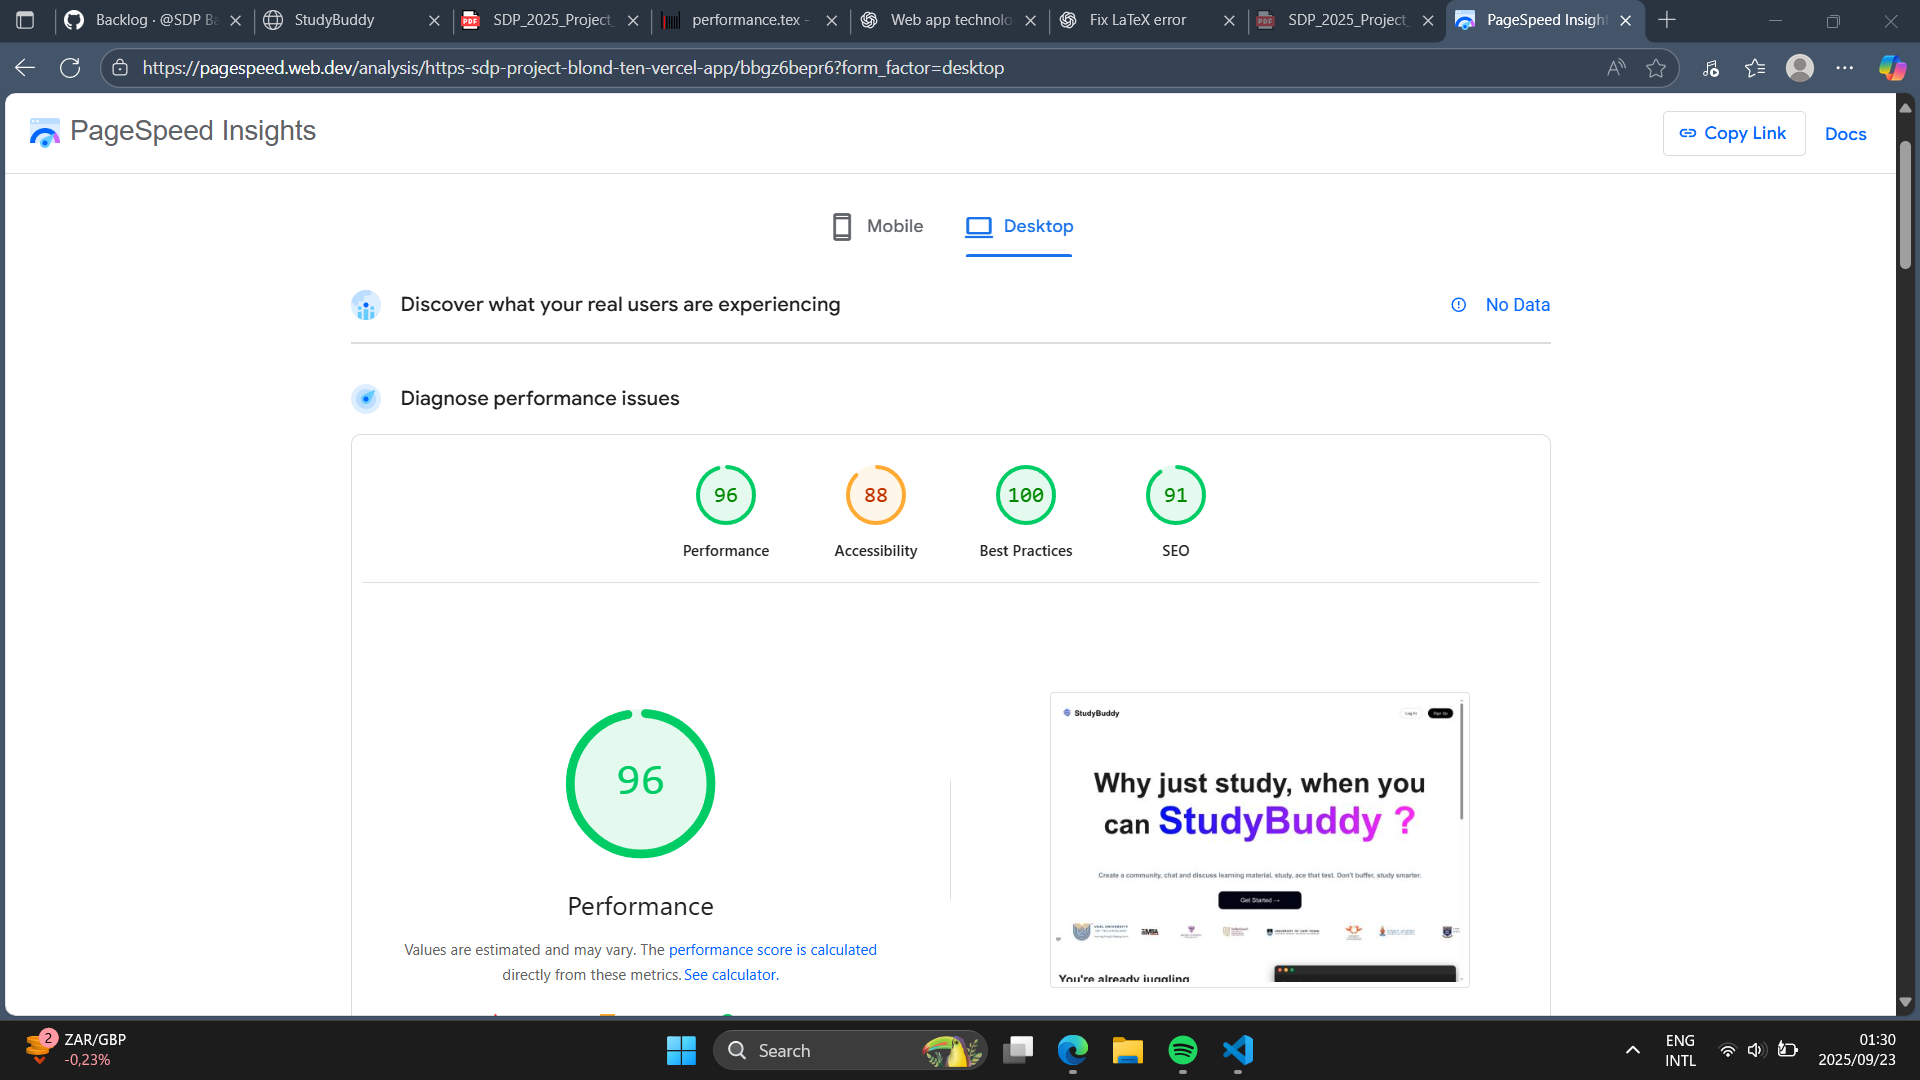
\includegraphics[width=0.8\textwidth]{desk.png}
    \caption{How Study Buddy performs on desktops}
    \label{fig:desktop_performance}
\end{figure}

\end{document}